% Drawing 86/02-6 -- folder 86, batch 02, archive page 29 (PDF page 30).
% Transcription: dans la marge gauche, en bas : un pentagone de sommets $t$ (en haut), $u$, $v$, $\tilde{u}$, $\tilde{v}$, dont le centre $s$ est joint aux cinq sommets ; à droite un carré de sommets $u$, $v$, $\tilde{u}$, $\tilde{v}$, le côté gauche $\{u, \tilde{v}\}$ épaissi et marqué $\Omega$, un point marqué au milieu du côté du haut et du côté du bas.
% Kind: pentagon with its centre joined to the vertices; square with one heavy side marked Omega. Method 2 (schematic redraw from the facsimile). Status: ok.
% Notes: Pentagon: the five sides between the same five vertices (t at the top, u and v at the sides, u-tilde and v-tilde at the bottom), the five spokes from the centre, the letter s under the centre; on the page the spokes stop short of the centre, where the letter stands, and are drawn here to one point just above it. Square: four sides between the same corners, the left side heavy with Omega at its left, a full point on the top side and one on the bottom side; corner letters u (upper left), v (upper right), u-tilde (lower right), v-tilde (lower left). Left out: the sketch of the diagram of p. 31 above (a typeset relation, not a drawing) and the struck figures between (drawing 02-5). Agrees with the transcription's note. Redrawn 2026-11-12 (issue 128): to check again.
% Coordinates: 1 unit = 1 mm = 1/100 of the crop width (bbox in page fractions: [0.1, 0.76, 0.4, 0.86]).
% Redrawn by Claude (claude-fable-5-2), issue #128, 2026-11-12; not checked by a human; not compiled (no TeX in the session).
% Rights: reproduces part of the work -- behind RENDER_TRANSCRIPTS, never published by itself.
\documentclass[tikz,border=3pt]{standalone}
\usepackage{amsmath,amssymb}
\usetikzlibrary{patterns,arrows.meta}
\tikzset{pencil/.style={black!45}, struck/.style={black!35}, mpt/.style={circle,draw,inner sep=1.3pt}, pt/.style={circle,fill,inner sep=0.9pt}, opt/.style={circle,draw,fill=white,inner sep=1.1pt}}
\begin{document}
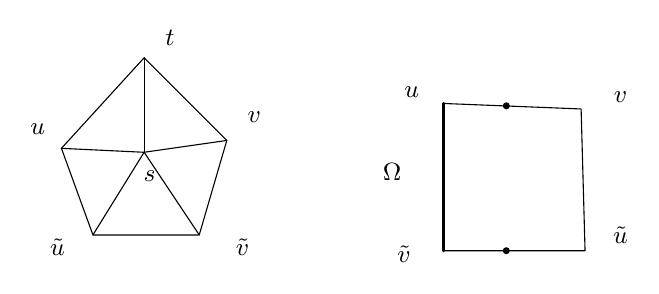
\begin{tikzpicture}[x=1mm,y=1mm,line cap=round,line join=round,font=\scriptsize]
\draw (34,-13.2) -- (44.5,-23.7) -- (41,-35.7) -- (27.5,-35.7) -- (23.5,-24.7) -- cycle;
\draw (34,-25.2) -- (34,-13.2);
\draw (34,-25.2) -- (44.5,-23.7);
\draw (34,-25.2) -- (41,-35.7);
\draw (34,-25.2) -- (27.5,-35.7);
\draw (34,-25.2) -- (23.5,-24.7);
\node[inner sep=1pt] at (37.3,-10.7) {\small $t$};
\node[inner sep=1pt] at (20.5,-22.2) {\small $u$};
\node[inner sep=1pt] at (48,-20.7) {\small $v$};
\node[inner sep=1pt] at (23,-37.2) {\small $\tilde{u}$};
\node[inner sep=1pt] at (46.5,-37.2) {\small $\tilde{v}$};
\node[inner sep=1pt] at (34.7,-28.2) {\small $s$};
\draw (72,-19) -- (89.5,-19.7) -- (90,-37.7) -- (72,-37.7);
\draw[very thick] (72,-37.7) -- (72,-19);
\node[pt] at (80,-19.3) {};
\node[pt] at (80,-37.7) {};
\node[inner sep=1pt] at (65.5,-27.7) {\small $\Omega$};
\node[inner sep=1pt] at (68,-17.5) {\small $u$};
\node[inner sep=1pt] at (94.5,-18.2) {\small $v$};
\node[inner sep=1pt] at (94.5,-35.7) {\small $\tilde{u}$};
\node[inner sep=1pt] at (67,-38.2) {\small $\tilde{v}$};
\end{tikzpicture}
\end{document}
